% Options for packages loaded elsewhere
\PassOptionsToPackage{unicode}{hyperref}
\PassOptionsToPackage{hyphens}{url}
\PassOptionsToPackage{dvipsnames,svgnames,x11names}{xcolor}
%
\documentclass[
  12pt]{article}

\usepackage{amsmath,amssymb}
\usepackage{lmodern}
\usepackage{iftex}
\ifPDFTeX
  \usepackage[T1]{fontenc}
  \usepackage[utf8]{inputenc}
  \usepackage{textcomp} % provide euro and other symbols
\else % if luatex or xetex
  \usepackage{unicode-math}
  \defaultfontfeatures{Scale=MatchLowercase}
  \defaultfontfeatures[\rmfamily]{Ligatures=TeX,Scale=1}
\fi
% Use upquote if available, for straight quotes in verbatim environments
\IfFileExists{upquote.sty}{\usepackage{upquote}}{}
\IfFileExists{microtype.sty}{% use microtype if available
  \usepackage[]{microtype}
  \UseMicrotypeSet[protrusion]{basicmath} % disable protrusion for tt fonts
}{}
\makeatletter
\@ifundefined{KOMAClassName}{% if non-KOMA class
  \IfFileExists{parskip.sty}{%
    \usepackage{parskip}
  }{% else
    \setlength{\parindent}{0pt}
    \setlength{\parskip}{6pt plus 2pt minus 1pt}}
}{% if KOMA class
  \KOMAoptions{parskip=half}}
\makeatother
\usepackage{xcolor}
\setlength{\emergencystretch}{3em} % prevent overfull lines
\setcounter{secnumdepth}{5}
% Make \paragraph and \subparagraph free-standing
\ifx\paragraph\undefined\else
  \let\oldparagraph\paragraph
  \renewcommand{\paragraph}[1]{\oldparagraph{#1}\mbox{}}
\fi
\ifx\subparagraph\undefined\else
  \let\oldsubparagraph\subparagraph
  \renewcommand{\subparagraph}[1]{\oldsubparagraph{#1}\mbox{}}
\fi

\usepackage{color}
\usepackage{fancyvrb}
\newcommand{\VerbBar}{|}
\newcommand{\VERB}{\Verb[commandchars=\\\{\}]}
\DefineVerbatimEnvironment{Highlighting}{Verbatim}{commandchars=\\\{\}}
% Add ',fontsize=\small' for more characters per line
\usepackage{framed}
\definecolor{shadecolor}{RGB}{241,243,245}
\newenvironment{Shaded}{\begin{snugshade}}{\end{snugshade}}
\newcommand{\AlertTok}[1]{\textcolor[rgb]{0.68,0.00,0.00}{#1}}
\newcommand{\AnnotationTok}[1]{\textcolor[rgb]{0.37,0.37,0.37}{#1}}
\newcommand{\AttributeTok}[1]{\textcolor[rgb]{0.40,0.45,0.13}{#1}}
\newcommand{\BaseNTok}[1]{\textcolor[rgb]{0.68,0.00,0.00}{#1}}
\newcommand{\BuiltInTok}[1]{\textcolor[rgb]{0.00,0.23,0.31}{#1}}
\newcommand{\CharTok}[1]{\textcolor[rgb]{0.13,0.47,0.30}{#1}}
\newcommand{\CommentTok}[1]{\textcolor[rgb]{0.37,0.37,0.37}{#1}}
\newcommand{\CommentVarTok}[1]{\textcolor[rgb]{0.37,0.37,0.37}{\textit{#1}}}
\newcommand{\ConstantTok}[1]{\textcolor[rgb]{0.56,0.35,0.01}{#1}}
\newcommand{\ControlFlowTok}[1]{\textcolor[rgb]{0.00,0.23,0.31}{#1}}
\newcommand{\DataTypeTok}[1]{\textcolor[rgb]{0.68,0.00,0.00}{#1}}
\newcommand{\DecValTok}[1]{\textcolor[rgb]{0.68,0.00,0.00}{#1}}
\newcommand{\DocumentationTok}[1]{\textcolor[rgb]{0.37,0.37,0.37}{\textit{#1}}}
\newcommand{\ErrorTok}[1]{\textcolor[rgb]{0.68,0.00,0.00}{#1}}
\newcommand{\ExtensionTok}[1]{\textcolor[rgb]{0.00,0.23,0.31}{#1}}
\newcommand{\FloatTok}[1]{\textcolor[rgb]{0.68,0.00,0.00}{#1}}
\newcommand{\FunctionTok}[1]{\textcolor[rgb]{0.28,0.35,0.67}{#1}}
\newcommand{\ImportTok}[1]{\textcolor[rgb]{0.00,0.46,0.62}{#1}}
\newcommand{\InformationTok}[1]{\textcolor[rgb]{0.37,0.37,0.37}{#1}}
\newcommand{\KeywordTok}[1]{\textcolor[rgb]{0.00,0.23,0.31}{#1}}
\newcommand{\NormalTok}[1]{\textcolor[rgb]{0.00,0.23,0.31}{#1}}
\newcommand{\OperatorTok}[1]{\textcolor[rgb]{0.37,0.37,0.37}{#1}}
\newcommand{\OtherTok}[1]{\textcolor[rgb]{0.00,0.23,0.31}{#1}}
\newcommand{\PreprocessorTok}[1]{\textcolor[rgb]{0.68,0.00,0.00}{#1}}
\newcommand{\RegionMarkerTok}[1]{\textcolor[rgb]{0.00,0.23,0.31}{#1}}
\newcommand{\SpecialCharTok}[1]{\textcolor[rgb]{0.37,0.37,0.37}{#1}}
\newcommand{\SpecialStringTok}[1]{\textcolor[rgb]{0.13,0.47,0.30}{#1}}
\newcommand{\StringTok}[1]{\textcolor[rgb]{0.13,0.47,0.30}{#1}}
\newcommand{\VariableTok}[1]{\textcolor[rgb]{0.07,0.07,0.07}{#1}}
\newcommand{\VerbatimStringTok}[1]{\textcolor[rgb]{0.13,0.47,0.30}{#1}}
\newcommand{\WarningTok}[1]{\textcolor[rgb]{0.37,0.37,0.37}{\textit{#1}}}

\providecommand{\tightlist}{%
  \setlength{\itemsep}{0pt}\setlength{\parskip}{0pt}}\usepackage{longtable,booktabs,array}
\usepackage{calc} % for calculating minipage widths
% Correct order of tables after \paragraph or \subparagraph
\usepackage{etoolbox}
\makeatletter
\patchcmd\longtable{\par}{\if@noskipsec\mbox{}\fi\par}{}{}
\makeatother
% Allow footnotes in longtable head/foot
\IfFileExists{footnotehyper.sty}{\usepackage{footnotehyper}}{\usepackage{footnote}}
\makesavenoteenv{longtable}
\usepackage{graphicx}
\makeatletter
\def\maxwidth{\ifdim\Gin@nat@width>\linewidth\linewidth\else\Gin@nat@width\fi}
\def\maxheight{\ifdim\Gin@nat@height>\textheight\textheight\else\Gin@nat@height\fi}
\makeatother
% Scale images if necessary, so that they will not overflow the page
% margins by default, and it is still possible to overwrite the defaults
% using explicit options in \includegraphics[width, height, ...]{}
\setkeys{Gin}{width=\maxwidth,height=\maxheight,keepaspectratio}
% Set default figure placement to htbp
\makeatletter
\def\fps@figure{htbp}
\makeatother

\addtolength{\oddsidemargin}{-.5in}%
\addtolength{\evensidemargin}{-1in}%
\addtolength{\textwidth}{1in}%
\addtolength{\textheight}{1.7in}%
\addtolength{\topmargin}{-1in}%
\makeatletter
\makeatother
\makeatletter
\makeatother
\makeatletter
\@ifpackageloaded{caption}{}{\usepackage{caption}}
\AtBeginDocument{%
\ifdefined\contentsname
  \renewcommand*\contentsname{Table of contents}
\else
  \newcommand\contentsname{Table of contents}
\fi
\ifdefined\listfigurename
  \renewcommand*\listfigurename{List of Figures}
\else
  \newcommand\listfigurename{List of Figures}
\fi
\ifdefined\listtablename
  \renewcommand*\listtablename{List of Tables}
\else
  \newcommand\listtablename{List of Tables}
\fi
\ifdefined\figurename
  \renewcommand*\figurename{Figure}
\else
  \newcommand\figurename{Figure}
\fi
\ifdefined\tablename
  \renewcommand*\tablename{Table}
\else
  \newcommand\tablename{Table}
\fi
}
\@ifpackageloaded{float}{}{\usepackage{float}}
\floatstyle{ruled}
\@ifundefined{c@chapter}{\newfloat{codelisting}{h}{lop}}{\newfloat{codelisting}{h}{lop}[chapter]}
\floatname{codelisting}{Listing}
\newcommand*\listoflistings{\listof{codelisting}{List of Listings}}
\makeatother
\makeatletter
\@ifpackageloaded{caption}{}{\usepackage{caption}}
\@ifpackageloaded{subcaption}{}{\usepackage{subcaption}}
\makeatother
\makeatletter
\@ifpackageloaded{tcolorbox}{}{\usepackage[many]{tcolorbox}}
\makeatother
\makeatletter
\@ifundefined{shadecolor}{\definecolor{shadecolor}{rgb}{.97, .97, .97}}
\makeatother
\makeatletter
\makeatother
\ifLuaTeX
  \usepackage{selnolig}  % disable illegal ligatures
\fi
\usepackage[]{natbib}
\bibliographystyle{agsm}
\IfFileExists{bookmark.sty}{\usepackage{bookmark}}{\usepackage{hyperref}}
\IfFileExists{xurl.sty}{\usepackage{xurl}}{} % add URL line breaks if available
\urlstyle{same} % disable monospaced font for URLs
\hypersetup{
  pdftitle={Introductory Data Science: A Blueprint to Navigate Curricular, Pedagogical, and Computational Challenges},
  pdfauthor={Elijah Meyer; Mine Çetinkaya-Rundel},
  pdfkeywords={Data Science, Curriculum, Pedagogy},
  colorlinks=true,
  linkcolor={blue},
  filecolor={Maroon},
  citecolor={Blue},
  urlcolor={Blue},
  pdfcreator={LaTeX via pandoc}}


\begin{document}


\def\spacingset#1{\renewcommand{\baselinestretch}%
{#1}\small\normalsize} \spacingset{1}


%%%%%%%%%%%%%%%%%%%%%%%%%%%%%%%%%%%%%%%%%%%%%%%%%%%%%%%%%%%%%%%%%%%%%%%%%%%%%%

\date{April 3, 2023}
\title{\bf Introductory Data Science: A Blueprint to Navigate
Curricular, Pedagogical, and Computational Challenges}
\author{
Elijah Meyer\\
Department of Statistics, Duke University\\
and\\Mine Çetinkaya-Rundel\\
Department of Statistics, Duke University\\
}
\maketitle

\bigskip
\bigskip
\begin{abstract}
The text of your abstract. 200 or fewer words.
\end{abstract}

\noindent%
{\it Keywords:} Data Science, Curriculum, Pedagogy
\vfill

\newpage
\spacingset{1.9} % DON'T change the spacing!
\ifdefined\Shaded\renewenvironment{Shaded}{\begin{tcolorbox}[breakable, frame hidden, boxrule=0pt, enhanced, interior hidden, borderline west={3pt}{0pt}{shadecolor}, sharp corners]}{\end{tcolorbox}}\fi

\hypertarget{sec-course}{%
\section{The Course}\label{sec-course}}

Reader should want to continue reading by thinking ``this is something
that I would like to teach''

In the following sections, we describe our introductory data science
course, offered to predominantly freshman level students at Duke
University, titled Introduction to Data Science and Statistical Thinking
(STA199). Often, these students are (interested in / major + minor in /
description of typical student demographic). Students enrolling in
STA199 commonly have little to no statistics, data science, or coding
experience. In a typical semester, this course seats roughly 179
students, which is considered to be large by all measures. Both the lack
of experience and large class size are identified as two common hurdles
by faculty when trying to create and instruct an introductory data
science course \citep{Schwab2020, Kok_2008}. However, by the end of this
course, students are able to use data both R and GitHub to create data
visualizations, investigate patterns, and model outcomes in a
reproducible format.

This course is built on four large-scale learning objectives: learn to
explore, visualize and analyze data in a reproducible and shareable
manner; gain experience in data wrangling and munging, exploratory data
analysis, predictive modeling, and data visualization; work on problems
and case studies inspired by and based on real-world questions and data;
learn to effectively communicate results through written assignments and
project presentation. These objectives are accomplished through
interactive lectures and labs that present content, problems, and case
studies inspired by and based on real-world questions and data.

When teaching, instructors are committed to the Kaplan Way learning
model (Figure 1) ``that combines a scientific, evidence-based design
philosophy with a straightforward educational approach to learning''
\citep[pg. 3]{schweser_2023}.

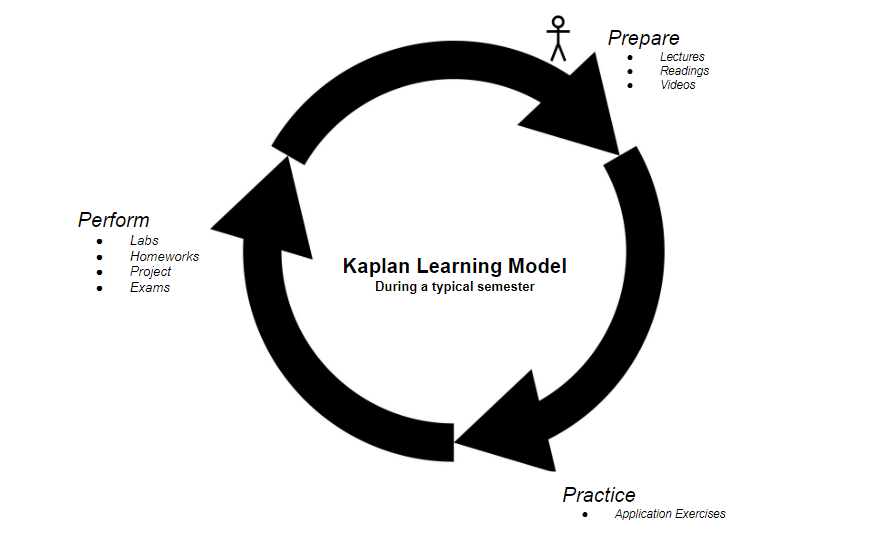
\includegraphics{images/Kaplan.png} \textbf{Fig 1:} Kaplan Learning
Model for STA 199

This model is composed of three phases: prepare, practice, and perform.
All three phases are designed to guide the instructor in facilitating an
overall quality learning experience for the student. Each of these
phases are performed during a typical week within a semester,
accomplished through preparation materials, lectures, in-class
application exercises, labs, and assessments.

During the prepare phase, students are completing readings, watching
videos, and listening to in-class lecture that ultimately helps
students' develop a new foundation of data science concepts being
learned. The goal of preparing students is to put them in a position
where they can build upon what they are learning, and create new
knowledge through the practice phase. The practice phase is designed to
be an opportunity for students to reinforce the new information gained,
as well as uncover new concepts in data science. This is achieved
through the use of interactive application exercises (AEs) administered
in class where students either work alone, in groups, or with the
instructor in live coding sessions. Finally, students enter the perform
phase, showcasing their progress made in the previous two phases. This
is typically done through assessments such as homework, labs, exams, and
projects. This learning model is a continuous cycle throughout the
semester as new topics are introduced.

Topics taught in STA199 fall under two major units: Unit 1 - Exploring
data; Unit 2 - Making rigorous conclusions. In Unit 1, students become
first introduced to R, R-studio, and Github. During this unit, students
start to create data visualizations and learn how to both import and
manipulate data to be better suited for analysis. In Unit 2, students
extend their investigations with data to include modeling. Specifically,
students fit a variety of models (simple linear regression, multiple
linear regression, logistic regression), and learn the fundamentals of
hypothesis testing. For a more complete description of the topics taught
and data sets used in creating these lessons, please see \textbf{A fresh
look at introductory data science (cite)}.

In this paper, we describe the preparation and implementation process of
STA199 in its entirety. This includes details of the teaching team used
to instruct, technology chosen to use when creating and implementing
STA199, and the pedagogical choices that go into a typical week of
teaching. We detail a comprehensive description of a flexible framework
on how to create, set up, and implement an introduction to data science
course similar to STA199. When describing this framework, we articulate
first hand experiences and suggestions surrounding some of the choices
made to create and instruct STA199. Throughout this paper, we aim to
support newer instructors who are developing or teaching an introductory
data science course; instructors with courses that are increasing in
size; and instructors who want to implement more technical tools into
their curricula and classroom.

\hypertarget{teaching-team}{%
\section{Teaching Team}\label{teaching-team}}

To account for the large class size, we structure and organize a
teaching team to best facilitate STA199. Our teaching team as a group
consists of one instructor and multiple teaching assistants (TAs). The
responsibilities of any TA is to both support the instructor in charge
of the class, and support the students in the classroom. These TAs range
from undergraduate to PH.D. level students, and vary in teaching
experience. \textbf{(Writing on TA selection process). Once
selected\ldots{} (writing on TA training).}

Once training is complete, TAs are assigned roles that indicate their
responsibilities during the semester. These roles include \emph{course
organizer}, \emph{head TA}, \emph{lab leader}, and \emph{lab helper}.
Often, these roles are given based on the academic level of student,
with more academically experienced TAs taking on the roles of course
organizer, head TA, and lab leader, where as students with less
experience (i.e.~undergraduate students) take on the role of lab helper.

Lab sections are held once a week, and are facilitated in person by both
a lab leader and lab helper. The responsibilities of a lab helper are
supporting both the students and lab leader as they see fit. Examples of
this may include setting up the classroom before class, or conducting
small group conversations when students have questions about the
material. The lab leader is responsible for facilitating the lab. This
involves working through a pre-made lab to ensure they can help students
apply concepts discussed in lecture to what's being assigned. In
addition, both must hold two hours of office hours each week and have
grading responsibilities assigned throughout the semester.

Head TA responsibilities can generally be categorized into the following
categories: Administrative and Pedagogical. Administrative
responsibilities include the organization and distribution of TA
responsibilities throughout the semester. It is imperative that the head
TA and instructor clearly communicate expectations with each other to
establish exactly how rules and responsibilities that are given to the
TAs are assigned. Other administrative duties include reminding other
TAs about bi-weekly payroll deadlines and ensure TAs are working their
alloted hours per week (and not more). Within these alloted hours, a
head TA distributes grading assignments and deadlines to both lab
helpers and leaders per week. The head TA makes sure that all TAs
complete grading within a week and spot check the grading accuracy and
quality of all written feedback given. We have had positive experiences
in having a head TA delegate administrative tasks to other members of
the teaching team. Pedagogically, head TAs are responsible for creating
or reviewing answer keys and grading rubrics for homework and lab
assessments as the instructor sees fit. Each head TA is also assigned to
instruct one lab section during the semester. Before becoming a Head TA,
there is additional training that specializes head TAs in their
administrative responsibilities.

The course organizer is expected to work across each section of STA199,
instead of working with a single instructor. Their responsibilities
include creating rubrics for and working through homework and lab
assignments. Additionally the course organizer, along with the
instructor, answers real time questions virtually during labs from lab
leaders. Questions often range from content related to technical
questions about GitHub and R. Finally, the course organizer is
responsible for handling all requested assignment extension requests
from students. This includes filing away student exemptions, providing
extensions for extreme circumstances, and enforcing the late work policy
outlined in the syllabus when necessary.

Although this is our proposed team structure, we want to emphasize that
there is great flexibility in coming up with how a teaching team is
built and operates for an introductory to data science course. Among any
team, we encourage a system designed to alleviate the grading
responsibilities of a large class from a single individual, dispersed
into many among the team. When grading, it is suggested that each
individual is properly trained on how to grade assessments, and
expectations on how to provide feedback are clear. This has often been a
point of contention from students in the past. For each assignment, we
recommend having one person grade one problem across the entirety of the
class roster. This helps adhere to more consistent grading, and
encourages more grading questions to be asked when they arise earlier in
the grading process.

Through our experiences, it has been imperative that everyone within the
team is communicating with each other. A team with many different roles
poses risk for the instructor to be unaware of how or what decisions are
being enacted at the grading and lab levels of the course. Thus, it is
recommended that the instructor trains everyone on the teaching team to
use a communication system that allows every member to communicate any
questions they may have, or decisions they make to the entire team. In
the past, we have used the software \emph{Slack}, with appropriately
named channels such as \emph{grading-questions} where TAs can post
examples and questions about grading and the instructor can clearly
state their expectations in a response. Further, it should be noted that
the head TA should not be treated as a ``bridge of communication'' for
the instructor to the rest of the teaching team. It is critical that
that the instructor is in consistent contact with all members of the
teaching team in making sure all lab leaders and helpers understand the
course content, upcoming assignments, and know what's expected of them
in their assigned role. We recommend holding a weekly meeting with all
members of the teaching team to ensure this. When members are unable to
come, it is an expectation that they watch a recorded video of the
meeting and reach out if they have any questions about what was
discussed.

\hypertarget{sec-tech}{%
\section{Technology}\label{sec-tech}}

In this section we will detail the computing infrastructure used to
create STA199. This includes details and examples with R, R-studio, and
GitHub, from the instructor's perspective, to set up lectures, AEs, labs
and homework. First, we start with the necessary student information to
collect before creation can take place.

\hypertarget{setting-up-a-github-account}{%
\subsection{Setting up a GitHub
account}\label{setting-up-a-github-account}}

We can use R, R-studio, and GitHub to create interactive lessons, and
assign pre-created assessments to individual or groups of students. To
do so, we must instruct students to create a GitHub account. This is
done of the first day of class, and often, students are given time
during class to sign up. Following tips from ``Happy Git with R''
(cite), we suggest students do the following when creating their name:

-- Incorporate your actual name

-- Reuse your username from other contexts if you can

-- Pick a username you will be comfortable revealing to your future boss

-- Be as unique as possible in as few characters as possible. Shorter is
better than longer

-- Avoid words with special meaning in programming (i.e., NA)

Once students create their account, we suggest getting this information
from them in a survey. This normally can be done through your learning
management system. It is critical to reiterate to students that spelling
and capitalization matter when answer this question. We suggest asking
the question as follows:

\begin{figure}

{\centering 
\includegraphics{images/github.question.png}

}

\end{figure}

If you, as the instructor, do not have a GitHub account, you will need
to create one as well. This student information will be needed to create
your GitHub organization for your course.

\hypertarget{github-organization}{%
\subsection{GitHub organization}\label{github-organization}}

GitHub organizations are shared accounts where instructors and students
can collaborate across many projects at once. Using your account, you
can create a new GitHub organization by clicking on your profile icon in
the upper right hand corner, go to \emph{Settings}, \emph{Access},
\emph{New Organization}. It's suggested to name this organization the
name of your class and the current semester you teaching in (i.e.,
sta199-s23). One of the many benefits of teaching through GitHub is the
ability to re-use what you currently create as a template for subsequent
semesters. Once your organization is created we can use packages within
R and R-studio to efficiently invite students and create assessments for
them.

\hypertarget{setting-up-r-r-studio}{%
\subsection{Setting Up R \& R-Studio}\label{setting-up-r-r-studio}}

R is a statistical programming language for computing, modeling, and
data visualization, while R-studio is an integrated development
environment for R (cite). Both are freely available to download and use.
In an introductory course, it is recommended to minimize student
frustration and distraction through the use of pre-packaged
computational infrastructure (Çetinkaya-Rundel and Rundel, 2018). Per
this recommendation, STA199 has students use R and R-studio through a
\emph{Duke Container}. Duke containers provides instructors at Duke
university the opportunity to facilitate the use of different software,
such as R and R-studio, through an online container instead of needing
students to locally download both programs. Additionally, instructors
have the ability to manage and install packages students will need for
the semester, helping provide a neat and well organized starting
experience with a new statistical language. (insert discussion on how
this is done).

(Thoughts: Transition to R-studio cloud discussion? What alternatives
can instructors use to imitate Duke containers if this is something they
do not have access to at their university.)

\hypertarget{using-r-r-studio-to-manage-github-organization}{%
\subsection{Using R \& R-Studio to manage GitHub
organization}\label{using-r-r-studio-to-manage-github-organization}}

(insert discussion / how-to on ghclass): includes invitations.

(set the stage for writing on how to create repos for students is
subsequent sections \emph{which will be a good segway})

. . .

R, R-studio, and GitHub aids in the creation and implementation our data
science pedagogy. This includes the creation and distribution of
in-class AEs, lectures, labs, and assessments. In the following sections
we describe in detail both how to create, structure, and distribute
materials used in STA199.

\begin{figure}

{\centering 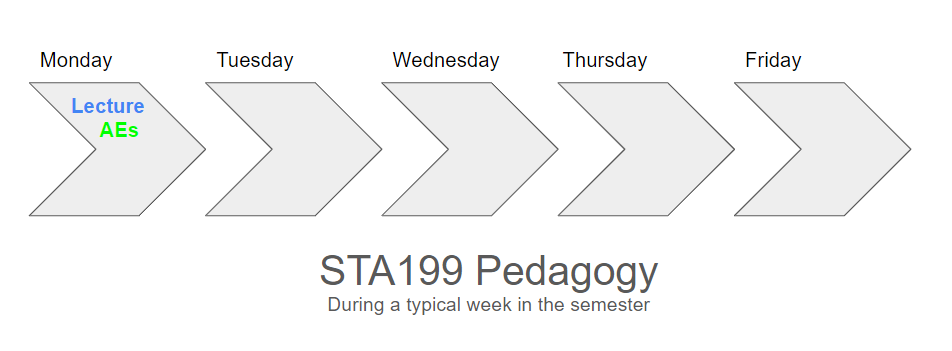
\includegraphics{images/pedagogy.png}

}

\end{figure}

\hypertarget{sec-ped}{%
\section{Pedagogy}\label{sec-ped}}

-- Reader should want to continue reading by thinking ``so how do I
teach this''

In this course, we have chosen a combination of teaching methods,
interactive activities, and learning assessments to help best prepare
introductory data science students the tools they need to be successful
outside of university or in future coursework. Our pedagogy includes
facilitating in-class AEs, facilitating lectures, running a lab, and
assigning assessments to provide students an opportunity to show what
they've learned.

\hypertarget{lecture}{%
\subsection{Lecture}\label{lecture}}

\hypertarget{application-exercies-aes}{%
\subsection{Application Exercies (AEs)}\label{application-exercies-aes}}

Application exercises are structured interactive lessons that allow
students to learn through doing in class. The purpose of these exercises
are to give students the opportunity to practice apply the statistical
concepts and code introduced in the prepare videos, readings, and
anything introduced during lecture. When first starting to create an AE,
we suggest streamlining the process through a GitHub template repository
cloned into R-studio as a project. We choose to use \emph{Quarto} within
R-studio to create AEs. This choice is intentional, to provide students
the opportunity to practice writing code and answering questions in a
reproducible format supported by such programming.

When creating an AE, we suggest creating a mix of guided and open ended
questions that encourage students to both follow along with instructor
demonstrations and progress to coding on their own. This format has
largely been accepted by students: ``I really enjoy the AE's and that
you take the time to walk us through the code and answer questions; I
like how the ae gives us a chance to practice the skills on our own
after class as well. Additionally, we suggest that questions are
scaffolded, meaning that if students fall behind or type incorrect code
when trying to follow along, that they have the ability to continuing
engaging for the remaining AE. This may include having answers to
questions in a separate document, or within the same AE towards the
bottom. Moreover, we suggest clearly labeling where students are
expected to type out answers in text or code throughout the exercise to
further streamline their involvement.

An example on an AE used to help teach (insert concept) can be found
here:

It is highly recommended to design lessons with built in time to have
students work on their own. The amount of time can largely depend on the
question being asked, and the teaching style of the instructor. We have
found that multiple 3-5 minute blocks for students to answer questions
without the instructor's guidance works well. Next, it is encouraged to
answer these questions together as a class built off student responses
before moving to the next set of material or questions.

We use the function \texttt{org\_create\_assignment} from the
\texttt{gh\_class} package to copy a template repository to students
whom are within the class GitHub organization. In order to create

(At this point in the paper, readers should know about github
organizations and information to collect from students. Don't let this
detail get lost to make this how-to section weaker)

\begin{Shaded}
\begin{Highlighting}[]
\FunctionTok{org\_create\_assignment}\NormalTok{(}
  \AttributeTok{org =}\NormalTok{ org,}
  \AttributeTok{repo =} \FunctionTok{paste0}\NormalTok{(assignment, }\StringTok{"{-}"}\NormalTok{, student\_name),}
  \AttributeTok{user =}\NormalTok{ student\_name,}
  \AttributeTok{source\_repo =} \FunctionTok{paste0}\NormalTok{(org, }\StringTok{"/"}\NormalTok{, assignment)}
\NormalTok{)}
\end{Highlighting}
\end{Shaded}

Above, \texttt{org} represents\ldots.

\texttt{assignment} is a character vector that represents the name of AE
to be copied to students (i.e.~ae-07);

\texttt{student\_name} is \ldots.

Talk about timing out issue?

Experience talking points:

\begin{itemize}
\item
  Invest time now so they can be re-tooled in future semesters
\item
  Talk about grading pros + cons
\item
  Talk about how AEs are the backbone of learning in this course (can
  not just lecture an expect to succeed)
\item
  Bring up how this works with a lot of students still
\end{itemize}

\hypertarget{labs}{%
\subsection{Labs}\label{labs}}

Labs for STA199 meet once a week for 75 minutes, and allow for students
to apply concepts found in prepare material, lecture, and AEs to various
data analysis scenarios. Lab section sizes are kept to around 30
students so each have more of an opportunity to converse with each other
and the lab leader when working through the assessment.

Much like AEs, the instructor or head TA will create and clone a lab
repository to all students that has the assessment and any other
intangibles (like a data set) in it by changing the \texttt{assignment}
vector to contain the name of original lab repository. Roughly one-third
of the way into the semester, students are assigned to groups to
complete a class project. We suggest strategically assigning groups
based on a collection of the following information

\begin{itemize}
\tightlist
\item
\item
\item
\item
  \ldots{}
\end{itemize}

Additionally, from this point forward in the semester, we suggest having
all labs be completed as group work. Introducing group work during lab
can help students learn from different perspectives, practice their
communication skills, and improve their problem solving skills in the
context of statistics and data science. When groups are formed, they are
tasked to come up with a team name. This team name will be the name used
to create their team repositories for the remaining labs. To create team
repositories, we use the following collected information from students:
lab section; team name; last name; first name. Please visit (insert
link) to see an example of the format explained. Note, these are fake
student names and have no meaning or association with Duke University.

We can use these data and change the code found in (figure-1??) to
create repositories for each team.

\begin{Shaded}
\begin{Highlighting}[]
\NormalTok{teams }\OtherTok{\textless{}{-}} \FunctionTok{read\_csv}\NormalTok{(}\StringTok{"teams.csv"}\NormalTok{)}

\FunctionTok{org\_create\_assignment}\NormalTok{(}
  \AttributeTok{org =}\NormalTok{ org, }\CommentTok{\# name of your organization}
  \AttributeTok{repo =} \FunctionTok{paste0}\NormalTok{(assignment, }\StringTok{"{-}"}\NormalTok{, teams}\SpecialCharTok{$}\NormalTok{team), }\CommentTok{\#name of the repo you are cloning and teams you are cloning for}
  \AttributeTok{user =}\NormalTok{ teams}\SpecialCharTok{$}\NormalTok{Github\_Username, }\CommentTok{\#adding individual students to team repo}
  \AttributeTok{team =}\NormalTok{ teams}\SpecialCharTok{$}\NormalTok{team, }\CommentTok{\#team (or group) they are added to}
  \AttributeTok{source\_repo =} \FunctionTok{paste0}\NormalTok{(org, }\StringTok{"/"}\NormalTok{, assignment) }\CommentTok{\#naming repo }
\NormalTok{)}
\end{Highlighting}
\end{Shaded}

The new expectation is that once groups are formed, one lab assessment
will be turned in for each group instead of each individual.

After groups are formed, we give a set of recommendations for groups to
help ensure a successful and positive group dynamic. This includes:

\begin{itemize}
\item
  Establish a clear line of communication with all members using Slack
  or another form of communication
\item
  Share ideas. Let your voice be heard.
\item
  Teach each other.
\item
  Do not approach group work as a bunch of individual assignments.
\end{itemize}

To further ensure positive group dynamic, we initiate three peer review
surveys. These peer review surveys provide \ldots\ldots{} Questions
range from only having instructor visibility, to being shared with all
team members to promote productive conversations. An example question is
as follows:

(insert example question)

Experience talking points for labs:

\begin{itemize}
\item
  Merge Conflicts (hesitancy to cause one)
\item
  Lots of work for large class sizes (groups)
\item
  Pros and cons of group formation
\item
  These are run by TAs (pros + cons)
\item
  Peer review question types
\end{itemize}

\hypertarget{assessments}{%
\subsection{Assessments}\label{assessments}}


\renewcommand\refname{Discussion}
  \bibliography{bibliography.bib}


\end{document}
